El experimento consistió en el uso de un difractómetro de rayos X \textit{BRUKER D2 PHASER}, en el cual se colocaba la muestra sólida sobre un portamuestras. En un principio, se realizó el barrido de la sal de mesa y la sal \textit{light}. 

Luego, se prepararon las muestras para las sales puras de KCl y KBr, así como sus soluciones. Estas últimas se formularon para distintos porcentajes molares, donde $X_{Br}$ representa la fracción molar de KBr y $X_{Cl} = 1 - X_{Br}$ la fracción molar de KCl. Las mezclas realizadas correspondieron a los siguientes porcentajes molares de KBr: 0\,\%, 20\,\%, 40\,\%, 60\,\% y 80\,\%.

Para la preparación de las soluciones, primero se colocaron las sales puras de KCl y KBr en vasos de precipitados y se calentaron durante aproximadamente 10 minutos sobre una platina calentadora. El objetivo de este paso fue evaporar la humedad residual que pudieran contener y así poder pesarlas con exactitud en una balanza de precisión (\textit{Insertar aquí el nombre de la balanza}) para obtener las proporciones molares deseadas. Una vez pesadas, las sales se combinaron en un vaso de precipitados y se disolvieron en agua destilada.

Las soluciones resultantes se dejaron reposar durante unos 5 días para permitir la evaporación del solvente y la posterior cocristalización. Como la evaporación natural no se completó debido a la humedad del ambiente, se aceleró el proceso colocando las muestras sobre una platina calentadora hasta evaporar la totalidad del agua, obteniendo así las muestras sólidas finales para su caracterización. Es importante destacar que la evaporación rápida del solvente no favorece un crecimiento cristalino ordenado, lo que dificulta la observación clara del proceso de cristalización en las muestras.

Adicionalmente, se preparó una solución pura de KBr mediante su disolución en agua destilada. Esta muestra se dejó evaporar a temperatura ambiente durante más de una semana con el objetivo de promover un crecimiento lento, obteniendo así cristales más grandes y ordenados que permitieran observar el proceso de cristalización con mayor claridad.

El equipo opera en geometría Bragg--Brentano, en la cual la muestra se encuentra en el centro del goniómetro y el sistema realiza un barrido $\theta$--$2\theta$, manteniendo la condición de incidencia y detección simétrica requerida para la difracción de rayos X.

\begin{figure}[htbp]
    \centering
    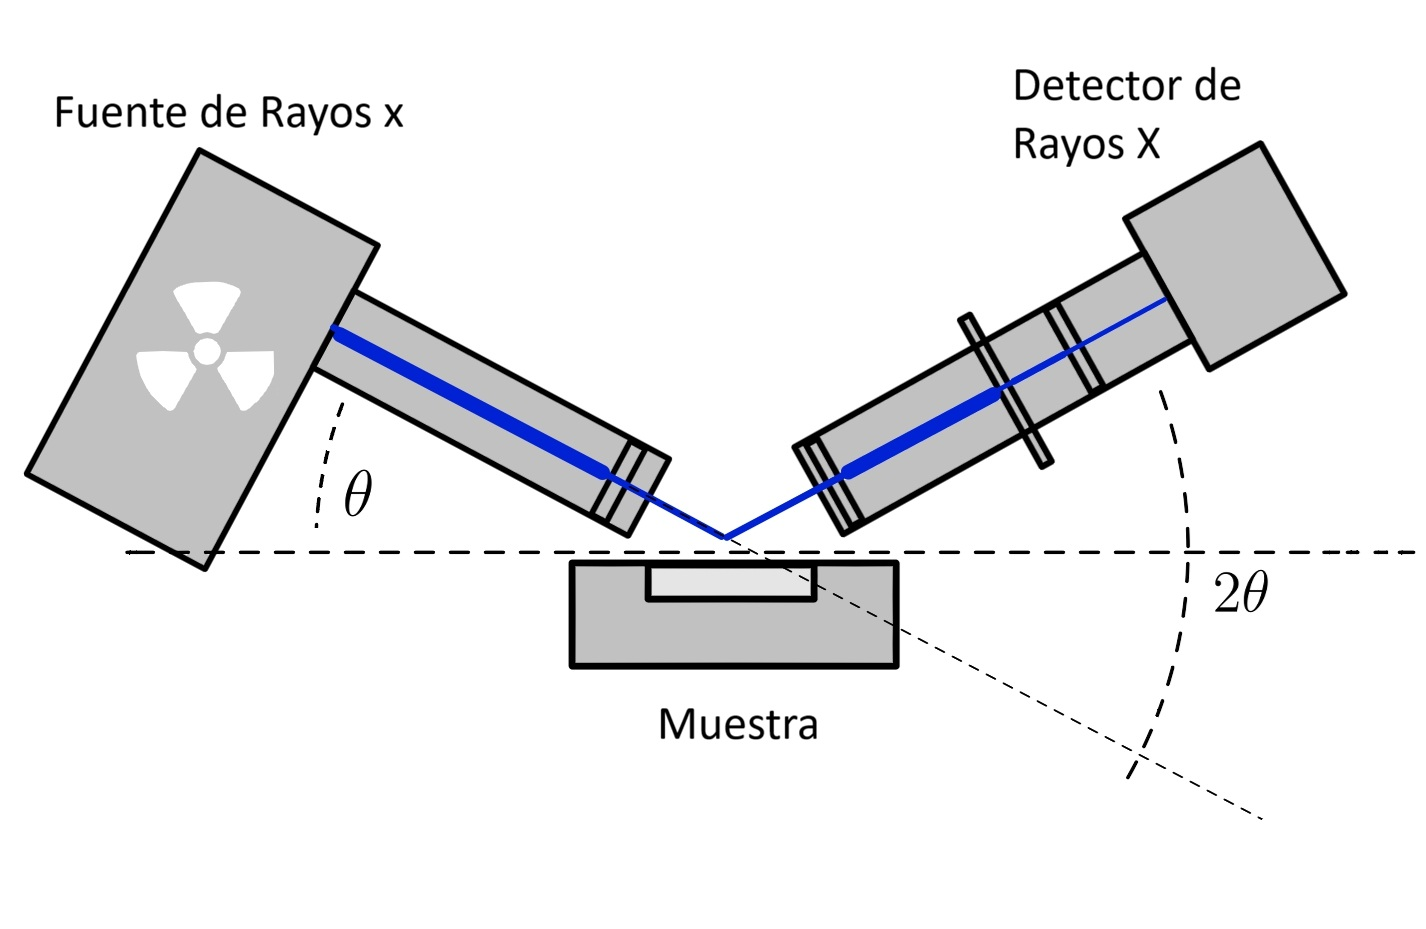
\includegraphics[width=0.5\textwidth]{Imagenes/esquema_difractometro.jpg}
    \caption{Esquema de la geometría Bragg--Brentano en configuración $\theta$--$2\theta$ para el difractómetro de rayos X.}
    \label{fig:bragg-brentano}
\end{figure}

Para la sal de mesa, se realizó un barrido en el rango de $10^\circ < 2\theta < 70^\circ$ con un paso de $0.02^\circ$ y un tiempo de conteo de 2 segundo por paso. Para las sales puras, sus soluciones, la sal \textit{light} y una mezcla con $X_{Br} = 0.6$, se realizó un barrido en el rango de $10^\circ < 2\theta < 80^\circ$ con un paso de $0.02^\circ$ y un tiempo de conteo de 2 segundos por paso.

El difractómetro mide los patrones de difracción irradiando la muestra con rayos X y detectando la intensidad de los rayos difractados en función del ángulo $2\theta$. Estos patrones se utilizan para identificar las fases presentes en la muestra, determinar su estructura cristalina y analizar la composición de las mezclas.

Se utilizó microscopía electrónica de barrido (\textit{SEM}) para observar la morfología de las muestras sólidas obtenidas tras la evaporación. Este análisis permitió evaluar el tamaño y la forma de los cristales formados, así como la presencia de posibles impurezas o defectos en la estructura cristalina.